%-----------------------------------------------------------------------------%
\chapter{\babTiga}
%-----------------------------------------------------------------------------%
Penulis menggunakan \textit{framework} FAST (\textit{Framework for the Application of Systems Thinking}) dalam mengembangkan aplikasi ini. FAST mendefinisikan tahapan untuk mengidentifikasi dan mengevaluasi permasalahan-permasalahan, kesempatan-kesempatan, hambatan-hambatan yang terjadi, dan kebutuhan yang diharapkan sehingga dapat diusulkan perbaikan-perbaikan \cite{susanto2013}. 

\noindent
Fase-fase pengembangan menggunakan FAST diilustrasikan seperti \pic~\ref{fig:fast} \cite{whitten2007}.

\begin{figure}
	\centering
	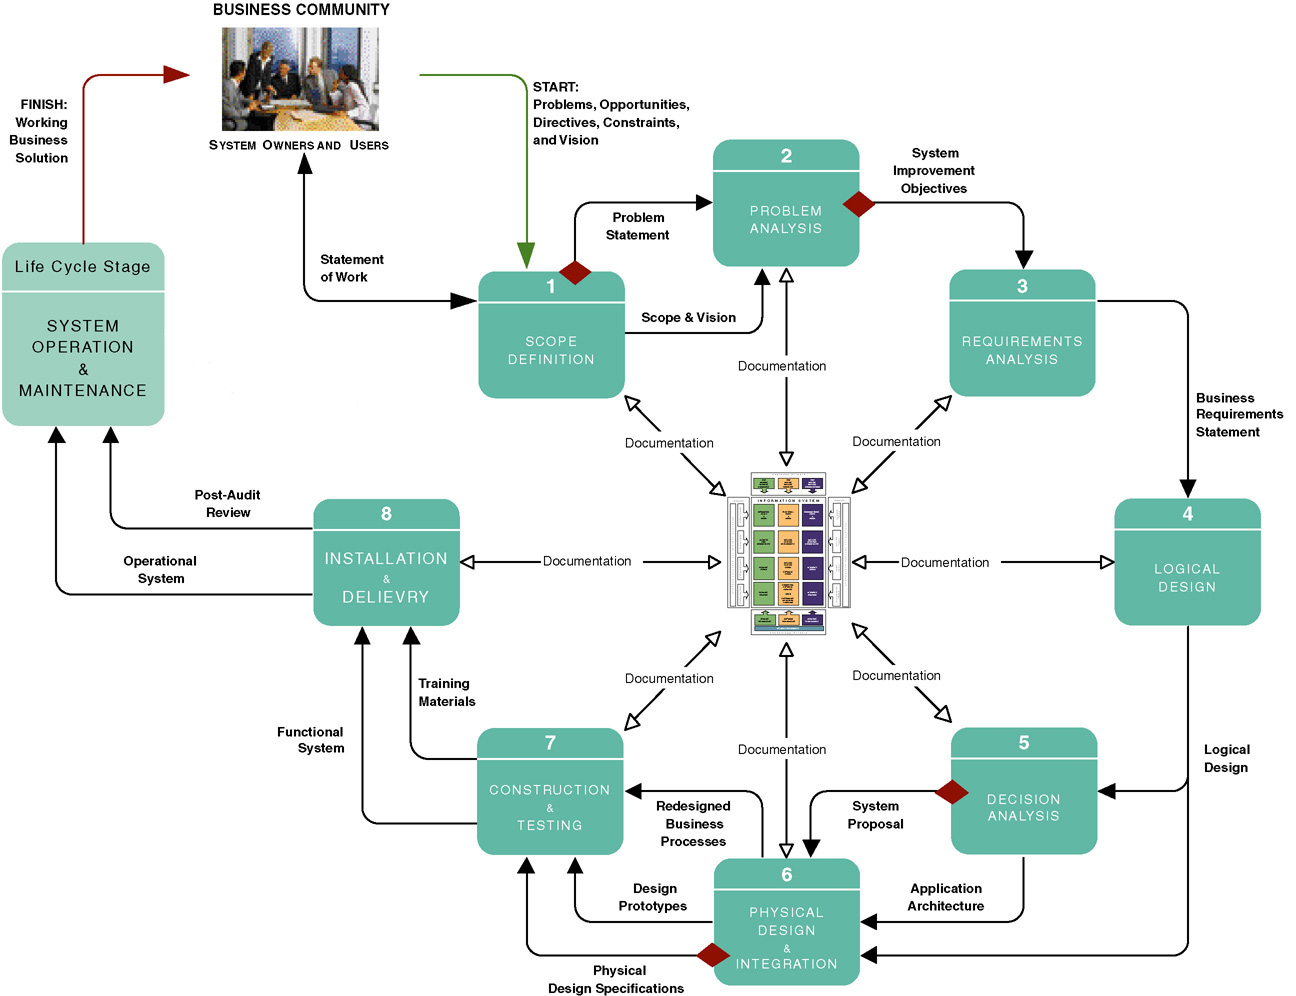
\includegraphics[width=1\textwidth]
		{pics/fastphase.jpg}
	\caption{Proses FAST framework}
	\label{fig:fast}
\end{figure}

\section{Definisi Lingkup}
Fase \f{scope definition} (definisi lingkup) ini digunakan untuk menetapkan  hal-hal sebagai berikut:

\begin{enumerate}[itemsep=-1ex]
\item Pernyataan masalah - pernyataan dan kategorisasi masalah, peluang dan arahan; juga dapat mencakup batasan dan visi awal untuk solusi, studi pendahuluan dan studi kelayakan.

\item Pembatas atau kendala - faktor pembatas yang mungkin membatasi solusi atau proses pemecahan masalah, termasuk di dalamnya besar anggaran, tenggat waktu, dan sumber daya manusia.

\item Pernyataan kerja - kontrak dengan manajemen dan komunitas pengguna untuk mengembangkan atau meningkatkan sistem informasi; mendefinisikan visi, ruang lingkup, batasan, kebutuhan pengguna, jadwal, dan anggaran.
\end{enumerate}

\section{Analisis Masalah}

Analisis masalah digunakan untuk mempelajari sistem yang ada  dan menganalisis temuan supaya tim proyek memiliki pemahaman yang menyeluruh tentang masalah yang memicu proyek.

Analis masalah sering mengungkap masalah baru dan menjawab pertanyaan yang paling penting, "Apakah manfaat dari pemecahan masalah ini melebihi biaya pembangunan sistem untuk memecahkan masalah ini?"

\section{Analisis Kebutuhan}

Analisis kebutuhan digunakan untuk menjawab pertanyaan-pertanyaan sebagai berikut: 
\begin{enumerate}[itemsep=-1ex]
\item Kemampuan apa yang harus disediakan sistem baru bagi penggunanya? 
\item Data apa yang harus ditangkap dan disimpan? 
\item Apa tingkat kinerja yang diharapkan? 
\item Apa prioritas dari berbagai kebutuhan?
\end{enumerate}

\section{Desain Logis}

Desain logis merupakan terjemahan dari kebutuhan pengguna bisnis ke dalam suatu model sistem yang menggambarkan hanya kebutuhan bisnis dan tidak ada desain teknis pelaksanaan kebutuhan tersebut. Desain ini meliputi desain konseptual dan desain penting. Model sistem adalah gambar sistem yang mewakili kenyataan atau realitas yang diinginkan. Model sistem memfasilitasi perbaikan komunikasi antara pengguna sistem, analis sistem, desainer sistem, dan pembangun sistem. 

Hal penting yang perlu diperhatikan juga pada tahap ini adalah pencegahan terjadinya \f{analysis paralysis}, sebuah istilah satir diciptakan untuk menggambarkan kondisi proyek umum di mana pemodelan sistem berlebihan secara dramatis memperlambat kemajuan menuju implementasi solusi sistem dimaksudkan.

\section{Analisis Keputusan}

Analisis keputusan digunakan untuk mengevaluasi kandidat sistem ditinjau berdasarkan:

\begin{enumerate}[itemsep=-1ex]
\item Kelayakan teknis: apakah solusi teknis praktis? Apakah staf kita memiliki keahlian teknis untuk merancang dan membangun solusi ini? 
\item Kelayakan operasional: apakah solusi yang memenuhi kebutuhan pengguna? Untuk tingkatan apa? Bagaimana solusi akan mengubah lingkungan kerja pengguna? Bagaimana pengguna mendapatkan manfaat dari solusi tersebut? 
\item Kelayakan ekonomi: apakah biaya solusi efektif? 
\item Jadwal kelayakan: dapatkah solusi dirancang dan dilaksanakan dalam waktu yang dapat diterima? 
\item Kelayakan Risiko: apa probabilitas keberhasilan implementasi menggunakan teknologi dan pendekatan?
\end{enumerate}

\section{Desain Fisik dan Integrasi}

Desain fisik merupakan terjemahan dari kebutuhan pengguna bisnis ke dalam suatu model sistem yang menggambarkan implementasi teknis kebutuhan bisnis pengguna. Sinonim umum termasuk desain teknis atau model implementasi. 

\noindent
Dua filosofi ekstrim desain fisik:
\begin{enumerate}[itemsep=-1ex]
\item \textit{Design by specification}: model sistem fisik dan spesifikasi rinci diproduksi sebagai rangkaian tertulis (atau yang dihasilkan komputer) cetak biru untuk konstruksi. 
\item \textit{Design by prototyping}: sistem tidak lengkap tetapi fungsi aplikasi dibangun dan disempurnakan berdasarkan masukan dari pengguna dan desainer lainnya.
\end{enumerate}

\section{Konstruksi dan Testing}
Fase pembangunan sistem yang meliputi: perangkat lunak, database, antarmuka sistem dan pengguna, perangkat keras, dan perangkat jaringan.

\section{Instalasi dan Penyerahan}
Fase instalasi dan penyerahan mencakup: instalasi sistem untuk dioperasikan yang sesungguhnya (\textit{production}), pelatihan pengguna, melengkapi dookumentasi, dan konversi data yang ada.